% The main text, shared by paper.tex (MLSys) and paper_ieee.tex (IEEE).
\section{Introduction}
Open-weight Mixture-of-Experts (MoE) models now carry 30--120\,B parameters and activate a few billion per token; a
desktop GPU has 24--32\,GB. Running such a model for one user therefore means keeping most experts in host DRAM. Each
decoded token reads its routed experts from GPU memory if they are resident, and otherwise from host memory: either the
CPU runs the expert, or the expert is copied over PCIe into a GPU slot \citep{ivanov2021datamovement,hoefler2021sparsity}.

Many systems build on this: GPU expert caches \citep{eliseev2023offloading,xue2024moeinfinity,song2024promoe}, CPU
execution of misses \citep{kamahori2024fiddler,ktransformers,zhong2025hybrimoe}, a per-miss choice between the
two \citep{freetoken,dali2026} and expert prediction \citep{hwang2024pregated,zhu2025preattention,wang2026seqmoe}. Each
reports a speed-up over a baseline of its choosing. None says how fast the same machine could decode the model, or which
part of the remaining time a better design could remove. Without that, a builder cannot tell whether to work on what is
cached, how it is read, when it is read, or how far ahead the routing must be predicted.

We answer these questions for batch-1 decode of gpt-oss-120b \citep{openai2025gptoss} and Qwen3-30B-A3B
\citep{yang2025qwen3} on rented RTX 5090 machines. We derive a bound, build oracles into a real engine that remove one
part of the gap at a time, and run them on many machines, with every prediction committed before its machine started.
\Cref{tab:claims} lists the answers and the evidence behind each.

\textbf{The headroom is large} (\cref{sec:limit}). MIN's host reads at the machine's probed rate bound the time per
token of any system with $C$ slots per layer, and that read time is nearly reachable in a microbenchmark. Our cache,
which leads FreeToken and llama.cpp at most configurations, runs at \dcShareMinLowMin--\dcShareMinLowMax\% of the
bound's speed at the smallest gpt-oss budget on machines with consumer processors; published systems, scored the same way, reach a median
\audInclassMed\%.

\textbf{What is cached and how it is read pay only together} (\cref{sec:gap}). In our engine, at the smallest gpt-oss budget, caching
MIN's set on the deployed read path, where the CPU serves a miss and a background copy fills its slot, closes almost none
of the gap; fetching the deployed set into its slots in the step closes none either. Doing both closes
\dmAllTogetherLow\% of the gap on \dmMachines{} panel machines, and \dmNewTogetherLow\% on \olN{} machines rented
later for a registered test. A registered control that issued the copies a step earlier failed its own check and ran
no faster. What the oracles leave we attribute to the GPU's own work in series with the reads and to the oracles' extra reads
(\cref{tab:gap}).

\textbf{Without foresight, little of it is reachable} (\cref{sec:online}). Four variants of the deployed cache built
from the engine's admission margin and its layer-ahead prediction recover at most \olCapLowMax\% of the read-ahead
oracle's gain on those machines: they read about as many experts as the deployed cache.

\textbf{The machine decides how foresight should be spent} (\cref{sec:foresight,sec:secondcard}). Each admitted
expert should be read once, with as few admissions as optimality allows, on the read path the link-to-CPU ratio
favours. A trend in that ratio, fitted on RTX 5090 machines, predicted the oracles' speed on \cxAllNWord{} RTX 4090
machines at ratios \cxAllRatioMin--\cxAllRatioMax{} within \cxAllDevLowMax\%; new RTX 5090 machines with fast links
scatter more around it.

\textbf{Foresight has a price} (\cref{sec:horizon}). Half of its value needs the routing of about \dcMed$\,C$ distinct
experts per layer ahead, on \fsModels{} models; exact routing of the next token recovers at most a third of it on our
workload.

\Cref{sec:builders} turns these results into rules for system builders; \cref{app:prereg,app:artifact} give
every prediction, including the failures, and the artifact.

\begin{table*}[!t]\centering\footnotesize
\caption{Our claims, the threshold registered for each before its machines started, and the result (\cref{app:prereg}
scores every clause). \emph{Derived}: follows from the definitions; \emph{post hoc}: found in the data it describes;
\emph{loose}: a threshold the earlier data made easy to meet; \emph{held}: the point estimate meets the threshold
(\cref{app:prereg} says which clauses also hold over their whole interval). \emph{Mach.}: machines that passed every
check; ``$a\,(b)+c$'': $a$ of the $b$ panel machines and $c$ new ones.}\label{tab:claims}
\setlength\tabcolsep{2pt}
\begin{tabular}{@{}>{\raggedright\arraybackslash}p{0.265\linewidth}>{\raggedright\arraybackslash}p{0.25\linewidth}>{\raggedright\arraybackslash}p{0.355\linewidth}r@{\hspace{3pt}}r@{}}\toprule
Claim & Registered threshold & Result & Mach. & \S \\\midrule
MIN's reads at the probed rate bound any exact-routing cache with $C$ slots per layer & derived & -- & -- & \ref{sec:limit} \\
The bound's read time is nearly reachable & $\ge$\,50\% of it per layer (loose) & \jdLayerMin--\jdLayerMax\%, held; \jdFailed{} of the job's \jdClauses{} clauses failed & \jdHosts & \ref{sec:limit} \\
Our cache is faster than FreeToken and llama.cpp at most configurations & on B: faster than FreeToken (interval $>$\,1), $\ge$\,1.8$\times$ llama.cpp ($\ge$\,2$\times$ at Qwen3 12.5\%); on S: within $\pm$0.06 of B's ratios & held on B; on S, \scRatioFailCells{} of six ratios fell outside $\pm$0.06 of B's; faster at \bothLeadCells{} of \bothCells{} in all & B, S & \ref{sec:limit} \\
MIN's set and one read pay only together (gpt-oss 11\%, fast links, greedy schedule) & interaction $>$\,0 on every machine; \MinOne's mean share of the gap 0.25--0.55 (loose) & positive on \dmRegHeld{} of \dmRegN{} panel machines (failed), \dmNewInteractionPosLow{} of \olN{} new ones (held; fast-link scope set in between); share \dmNewTogetherLow\% & \dmRegN\,(\dmMachines)${}+{}$\olN & \ref{sec:gap} \\
Issuing the copies a step earlier does not rescue the two-read path & misses $\le$\,0.95$\times$ \FewTwo's; slowdown $\le$\,0.01; per machine and budget & at 11\%: misses \tcMissRatioLowRng$\times$, \tcSlowLowRng{} slower; failed on \tcTOneFailed{} and \tcTTwoFailed{} of \tcTOneN{} machine-budgets; the second read costs more than the late landing (held) & \tcN & \ref{sec:gap} \\
Policies without foresight recover little of the oracle's gain & speed $\le$\,1.10$\times$; capture $\le$\,35\% (loose), per machine & best \olBestLowMin--\olBestLowMax$\times$, capture at most \olCapLowMax\% (held) & \olN & \ref{sec:online} \\
MIN's fewest-admission set read once gains on stable machines & $>$\,1 on every machine & \rbPlanMean$\times$ (geometric mean) on all \rbPlanMachines{} stable machines, held on the \rbPlanRegMachines{} registered; lost on the \rbPlanUnstLost{} unsteady ones (one registered, failed; one excluded by its job's validity rule) & \rbPlanMachines & \ref{sec:foresight} \\
The link-to-CPU ratio predicts the oracles' speed on a second card & within 0.10 in log of the RTX 5090 trend (trend fitted post hoc) & within \cxAllDevLowMax\% at ratios \cxAllRatioMin--\cxAllRatioMax{} (held); new fast-link RTX 5090s off by up to \olTrendDevMax\% (post hoc) & \cxAllN & \ref{sec:secondcard} \\
Our cache reaches \dcShareMinLowMin--\dcShareMinLowMax\% of the bound on consumer machines (gpt-oss 11\%) & post hoc; consumer scope set after the data & server machines: \dcShareServLowMin--\dcShareServLowMax\% & \dcMachinesLow & \ref{sec:limit} \\
Published systems reach a median \audInclassMed\% of their bound & post hoc & their papers' hardware at datasheet rates & -- & \ref{sec:limit} \\
Half of foresight's value needs $\approx$\dcMed$\,C$ distinct experts ahead & post hoc & on \fsModels{} models' traces & -- & \ref{sec:horizon} \\
\bottomrule
\end{tabular}
\end{table*}

\section{Setting}\label{sec:setting}
\paragraph{Models and workload.} gpt-oss-120b has 36 MoE layers of 128 experts, top-4, in MXFP4 (13.25\,MB per
expert). Qwen3-30B-A3B has 48 layers of 128 experts, top-8, in BF16 (9.44\,MB per expert). Prompts are AIME-25
problems, and the cache carries over between problems, as in one user's session. The system comparison decodes 256
tokens of each of the 30 problems through each system's server. The engine experiments replay the model's own greedy
output, teacher-forced, so that every configuration sees the same routing. A \emph{budget} is the share $C/E$ of each
layer's experts that fit in GPU slots: gpt-oss 11\% and 25\% are $C{=}14$ and $C{=}32$ of 128. The two smallest budgets
of each model are \emph{host-bound}: at the GPU's datasheet rate, host reads, not the GPU, limit their speed in
\cref{eq:limit}, except at gpt-oss 25\% on the few machines with the fastest host memory. At the GPU's measured batch-1
rate the GPU term also binds at gpt-oss 25\% on both hosts of \cref{tab:headline}, and at Qwen3 25\% on host B. Most results are at gpt-oss 11\% and
25\%.

\paragraph{The engine.} Our cache is a 3{,}500-line patch to llama.cpp \citep{llamacpp}. Each MoE layer has $C$ GPU
slots. A \emph{miss} is read from host memory in one of two ways: CPU helper threads run it, or it is \emph{fetched}
(copied into a slot over PCIe and run on the GPU in the same step). A per-machine table, computed from the machine's
bandwidth probe, sets how many of a layer's misses are fetched. The \emph{deployed} policy admits a miss into a slot
when its decayed request count beats the lowest resident's by a margin $\kappa{=}1$. The CPU serves the admitted miss
and a background copy then fills its slot, so the expert is read from host memory twice (\cref{fig:step}).

\begin{figure}[t]\centering
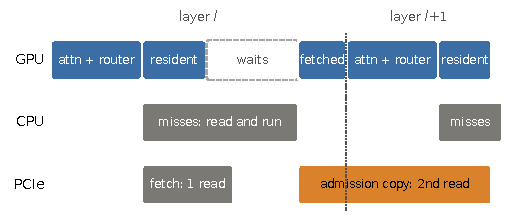
\includegraphics[width=\linewidth]{figs/step.pdf}
\caption{One decode step of the deployed cache, schematically. Blue: the GPU's own kernels. Grey: host reads of the
misses, which the step waits for. Orange: the background copy that fills an admitted expert's slot, a second read of
the same expert.}\label{fig:step}
\end{figure}

\paragraph{Terms.} \emph{MIN} is Belady's optimum with bypass \citep{belady1966study,bypassopt}: it \emph{admits} a miss
only if some resident is needed later than the miss, which gives the most hits possible with $C$ slots
\citep{carlisle1995kcoloring,jain2016hawkeye}. Many schedules reach that optimum. The \emph{greedy} one admits whenever
it may; the \emph{fewest-admission} one admits as rarely as any of them. An admitted expert is read \emph{once}
(\cfg{1R}), fetched into its slot in the step that needs it, or \emph{twice} (\cfg{2R}), served by the CPU in that step
and copied in the background; the engine publishes a background copy at the start of the second step after the one that
admitted it. A copy issued a few steps before the expert's use is read \emph{ahead}. \emph{Oracles} read the future
routing from a trace recorded on the same machine. Configurations are named by the set admitted and the number of reads: \MinOne{} is MIN's
greedy set read once, \MinTwo{} the same set read twice, \DepOne{} the deployed set read once, and \FewOne{} and \FewTwo{}
MIN's fewest-admission set. \Cref{tab:configs} lists the configurations, machine sets and yardsticks (the window policies of
\cref{sec:horizon} are in \cref{app:value}), and \cref{app:names} maps the codes of the appendix tables to these names.

\paragraph{Machines.} Every machine is a rented host with one RTX 5090 (an RTX 4090 in \cref{sec:secondcard}). Each
runs our bandwidth probe before any model run. It reads host memory from CPU threads, at the number of helper threads
the engine uses ($B_c$), and over PCIe into the GPU, at the rate the engine's copies use ($B_p$); $B_{\mathrm{host}}$ is
its highest reading by any method. The \emph{link-to-CPU ratio} is $B_p/B_c$. We call a link \emph{fast} when the ratio
is at least 0.5 and \emph{slow} otherwise; the term compares the link with the CPU, not with other links, and we drew
the 0.5 line after the panel's data, before the registered tests of \cref{sec:gap,sec:online,sec:secondcard}. Ryzen, Core and
Threadripper parts, high-end desktop ones included, are \emph{consumer} processors; EPYC, Xeon and engineering-sample
parts are \emph{server} processors.

\begin{table}[t]\centering\footnotesize
\caption{Cache configurations. \emph{Reads}: how many times an admitted expert is read from host memory. All run in the
same engine; the oracles read the future routing from a trace of the same text recorded on the same machine.}\label{tab:configs}
\setlength\tabcolsep{3pt}
\begin{tabular}{@{}p{0.27\linewidth}p{0.57\linewidth}c@{}}\toprule
Name & What it admits, and how & Reads \\\midrule
\multicolumn{3}{@{}l}{\emph{No foresight}} \\
deployed & decayed request count beats the lowest resident's by $\kappa{=}1$; the CPU serves the miss, then a background copy fills the slot & 2 \\
single read & the same admissions, fetched into the slot in the step & 1 \\
admit every miss & every miss fetched into the lowest-scored slot (demand fetch) & 1 \\
\midrule
\multicolumn{3}{@{}l}{\emph{Oracles}} \\
MIN, 2 reads & MIN with bypass (greedy rule); the CPU serves the miss, then a copy & 2 \\
MIN, 1 read & MIN with bypass (greedy rule); admissions fetched in the step & 1 \\
MIN, fewest adm. & the hit-optimal schedule with the fewest admissions (an LP per host), with 2 or 1 reads & 2 or 1 \\
MIN, prefetched & MIN, 1 read, plus copies issued three steps ahead & 1 \\
Belady & every expert of the coming steps, into the slot needed furthest ahead (also with 1 read, and prefetched) & 2 or 1 \\
window $W$ & admit every miss unless the next $W$ tokens show the victim needed sooner; victim the lowest-scored resident not seen in the window, else the one seen furthest & 1 \\
window $W$, recall $r$ & the same, each future expert kept with probability $r$, else replaced by a random one & 1 \\
deployed + window $W$ & the deployed policy with the same window and victim choice; the CPU serves the miss, then a background copy & 2 \\
\bottomrule
\end{tabular}
\end{table}


\paragraph{Statistics and registration.} Time per token is averaged over problems, and speed ratios are ratios of mean
times. Machines differ far more than problems (two panel machines with the same CPU model differ by up to
\pnSameCpuDiffMax\% in the deployed cache's time), so the machine is the unit. Claims are about orderings that hold on every machine of a stated class, and
summaries over machines carry 95\% $t$-intervals over machines, since with a handful of machines a percentile bootstrap over machines is too narrow \citep{kalibera2013rigorous}; comparisons on one machine carry 95\% intervals over problems (a paired bootstrap). A \emph{launch} is one rental; in
the later experiments each configuration ran in two or three processes, \emph{rounds}, per launch (at 25\% in the
registered tests, one). A machine
\emph{ran stably} when its outputs matched the reference and, where it ran more than one process, their times agreed
within 2\%; two experiments ran each configuration in a single process, so only the first condition applies to them (\cref{app:prereg}). Intervals over problems leave out rounds and rentals: a speed ratio moved by a median \nzRoundMed\% (at most
\nzRoundMax\%) between rounds and \nzRentalMed\% (at most \nzRentalMax\%, where a relaunch's probe changed the fetch
table) between rentals. Widened by its round range, each of the \nzHeldCI{} per-machine registered clauses that held
with an interval still does; widened by the largest rental difference, \nzRentalStillHeld{} do, and
\nzRentalMovedNarrow{} of the other \nzRentalMoved{} are bands of $\pm$0.06 or narrower (\cref{app:prereg}). Every
experiment's predictions were committed to a public branch before its machine started; \cref{app:prereg} scores all of
them, and \cref{tab:claims} marks the thresholds that earlier data made easy to meet.

\section{How Fast Could It Be?}\label{sec:limit}
Consider any system that executes the model's exact routing with at most $C$ experts of each layer resident on the
GPU. Per token, each of the $Lk$ routed experts is served by a resident copy or read from host memory. Let $R^\star$ be
MIN's host reads per token, summed over layers, on the routing trace the engine runs (\cref{app:artifact}); no policy,
even one that knows the future, reads fewer. If $m$ experts
per token run on the CPU, host memory supplies at least $\max(R^\star,m)\,S$ bytes for experts of $S$ bytes, and the GPU
reads the dense weights $D$ plus $(Lk-m)\,S$. With everything overlapped,
\begin{equation}
\bar T \;\ge\; \min_{0\le m\le Lk}\ \max\!\Big(\frac{D+(Lk-m)S}{B_{\mathrm{gpu}}},\ \frac{\max(R^\star\!,m)\,S}{B_{\mathrm{host}}}\Big).
\label{eq:limit}
\end{equation}
At a host-bound budget this is MIN's read time, $R^\star S/B_{\mathrm{host}}$. The bound assumes exact routing, whole
experts, at most $C$ residents per layer and one token per step. It drops all latencies, lets the two read paths share
$B_{\mathrm{host}}$, and is relative to the probe: a reader faster than the probe could beat it (\cref{sec:limits}).

\paragraph{The demand bound: reads that wait for the router.} A system that reads an expert only after its layer's router
has chosen it cannot overlap that read with the GPU's work: layer $l$'s misses are known only after its attention and
router, and layer $l{+}1$ starts only after layer $l$'s experts. Its time is at least the GPU's non-expert work plus the
reads, in series:
\begin{equation}
\bar T_{\text{demand}} \;\ge\; T_{\text{GPU}} + \frac{R^\star S}{B_{\mathrm{host}}},
\label{eq:demand}
\end{equation}
where $T_{\text{GPU}}$ is the GPU's attention, dense layers, norms and routers per token: \dmTgpu\,ms for gpt-oss, the
smallest of the \slProfN{} Nsight profiles of our engine we use; a system with faster non-expert kernels has a lower bound. Every system we compare reads on demand; only reads issued before routing can go below
\cref{eq:demand}.

\paragraph{The ordered bound: reads foresight cannot free.} Foresight does not free every read. An expert run on the CPU needs
its layer's attention output, and the next layer's attention needs its result, so CPU reads sit in series with the GPU's
non-expert work; only copies over the link can be issued ahead. This assumes that the CPU reads an expert's weights from
memory when it runs it; a read-ahead into the CPU's cache would relax it. With a share $f$ of MIN's reads served by the
CPU at the probe's highest CPU reading $\hat B_c$ and the rest copied at its highest link reading $\hat B_p$,
\begin{equation}
\bar T \;\ge\; \min_{0\le f\le 1}\ \max\!\Big(\frac{(1-f)\,R^\star S}{\hat B_p},\ T_{\text{GPU}} + \frac{f\,R^\star S}{\hat B_c}\Big),
\label{eq:dep}
\end{equation}
and \cref{eq:limit} holds as well, so the bound is the larger of the two.
On the median consumer machine at gpt-oss 11\%, \cref{eq:dep} equals \cref{eq:limit} (ratio \dcDepOverLimLowMed); where
the link is slow, it is up to \dcDepOverLimLowMax{} times as high.

\paragraph{The read time is nearly reachable.} A microbenchmark replays MIN's per-layer reads of gpt-oss on
\jdHosts{} machines without the model: CPU threads read part of each layer's experts while the copy engine copies the rest.
It reaches \jdLayerMin--\jdLayerMax\% of the bound's read time (\cref{tab:readsched}; registered: at least 50\%, a loose threshold). The GPU term of \cref{eq:limit} is
looser, but at datasheet rates it binds only at the largest budgets (\cref{tab:limit}).

\paragraph{Where systems stand.} \Cref{tab:headline} places three systems against the bounds on two machines. Our
cache leads FreeToken \citep{freetoken} at \bothLeadCells{} of \bothCells{} configurations and stock llama.cpp at all
of them (\cref{app:system}). Across \dcMachinesLow{} machines with consumer processors at gpt-oss 11\%, it runs at
\dcShareMinLowMin--\dcShareMinLowMax\% of the speed of \cref{eq:limit}, the bound we use throughout
(\dcShareDepLowMin--\dcShareDepLowMax\% of \cref{eq:dep}); the \olN{} machines added in \cref{sec:gap} fall at
\olShareLowMin--\olShareLowMax\%. The top of that range is probably too high: on that machine the engine's reads imply, by the closed-form
account of \cref{app:relation}, a rate above the probe's best reading (\cref{tab:robust}).

\paragraph{Published systems (post hoc).} Scored against the same bound on their papers' own hardware at datasheet
rates, \audInclassN{} published batch-1 measurements reach a median \audInclassMed\%; ours, scored the same way, a median
\audOursMed\% (\cref{app:audit}, which gives the caveats).

\begin{table*}[t]\centering\small
\caption{Decode speed at equal GPU expert memory on two RTX 5090 hosts. 30 AIME-25 problems, first 256 decode tokens,
greedy, session; our cache uses the FETCH split computed from each machine's bandwidth probe; FreeToken uses its faster
backend per budget, picked on listing B on a separate launch and carried over to the second host. Ratios are of mean
speeds, paired by problem, with 95\% bootstrap intervals. \emph{Speed limit}: the fastest any exact-routing system with
the same slots per layer can decode on that machine (\cref{sec:limit}: exact optimum, that host's highest probed rate,
datasheet GPU rate; \cref{tab:limit} tightens it). With every weight in the VRAM of an RTX PRO 6000 (the RTX 5090's
datasheet bandwidth, 96\,GB), stock llama.cpp decodes gpt-oss at 255 and Qwen3 at 178\,tok/s.
$^\dagger$Launch 1 for both systems: FreeToken's backend was picked on the launch it is scored on, which favours it,
and the row has no confirmation launch.}\label{tab:headline}
\resizebox{\textwidth}{!}{%
\begin{tabular}{llrrrcrrr}\toprule
Model & Experts & llama.cpp & FreeToken & Ours & Ours $\div$ FreeToken & Ours $\div$ & Speed & Ours, \% \\
 & on GPU & (tok/s) & (tok/s) & (tok/s) & (95\% CI) & llama.cpp & limit & of limit \\\midrule
\multicolumn{9}{l}{\textbf{Listing B}: Ryzen 9 9950X3D, card at 17001\,MHz memory clock, CPU 72\,GB/s, link 53, together 78} \\
gpt-oss-120b & 11\% & 34.9 & 54.0 {\scriptsize(hybrid)} & \textbf{69.9} & 1.294 [1.278, 1.312] & 2.00$\times$ & 172 & 41\% \\
gpt-oss-120b & 25\% & 40.0 & 85.6 {\scriptsize(hybrid)} & \textbf{109.2} & 1.275 [1.254, 1.295] & 2.73$\times$ & 430 & 25\% \\
gpt-oss-120b & 40\% & 47.7 & 132.2 {\scriptsize(offload)} & \textbf{152.5} & 1.154 [1.134, 1.172] & 3.20$\times$ & 519 & 29\% \\
Qwen3-30B-A3B & 12.5\% & 19.5 & 38.7 {\scriptsize(hybrid)} & \textbf{40.0} & 1.032 [1.022, 1.042] & 2.05$\times$ & 96 & 42\% \\
Qwen3-30B-A3B & 25\% & 22.1 & 54.7 {\scriptsize(hybrid)} & \textbf{63.1} & 1.153 [1.134, 1.173]$^\dagger$ & 2.86$\times$ & 214 & 30\% \\
Qwen3-30B-A3B & 43.75\% & 28.4 & 103.1 {\scriptsize(offload)} & \textbf{108.2} & 1.049 [1.036, 1.064] & 3.81$\times$ & 308 & 35\% \\
\midrule
\multicolumn{9}{l}{\textbf{Stock-clock host}: Ryzen 9 9950X, card at 14001\,MHz, CPU 56\,GB/s, link 53, together 66; FreeToken's backend carried over from listing B} \\
gpt-oss-120b & 11\% & 28.9 & 48.0 {\scriptsize(hybrid)} & \textbf{57.9} & 1.207 [1.195, 1.219] & 2.00$\times$ & 140 & 41\% \\
gpt-oss-120b & 25\% & 33.6 & 78.7 {\scriptsize(hybrid)} & \textbf{94.1} & 1.196 [1.163, 1.224] & 2.80$\times$ & 351 & 27\% \\
gpt-oss-120b & 40\% & 40.1 & 122.2 {\scriptsize(offload)} & \textbf{133.6} & 1.093 [1.077, 1.111] & 3.34$\times$ & 514 & 26\% \\
Qwen3-30B-A3B & 12.5\% & 16.1 & 32.7 {\scriptsize(hybrid)} & \textbf{33.5} & 1.027 [1.018, 1.036] & 2.08$\times$ & 78 & 43\% \\
Qwen3-30B-A3B & 25\% & 18.5 & 51.4 {\scriptsize(hybrid)} & \textbf{53.9} & 1.048 [1.037, 1.059] & 2.91$\times$ & 174 & 31\% \\
Qwen3-30B-A3B & 43.75\% & 23.8 & \textbf{98.3} {\scriptsize(offload)} & 95.8 & 0.974 [0.962, 0.987] & 4.02$\times$ & 305 & 31\% \\
\bottomrule\end{tabular}}\end{table*}


\section{Where the Seconds Go}\label{sec:gap}
The gap is the deployed cache's time beyond \cref{eq:limit}. Oracles in the engine remove three parts of it: what is
cached (MIN's set instead of the deployed one), how it is read (each admitted expert fetched once in the step, instead of
served by the CPU and copied in the background), and when (the read-ahead oracle issues its copies a few steps early). We change the first two alone and together, on the
\dmMachines{} panel machines that ran every state and, under a test registered before they started, on \olN{} machines
rented for it (\cref{fig:staircase,tab:gap}).

\begin{figure*}[t]\centering
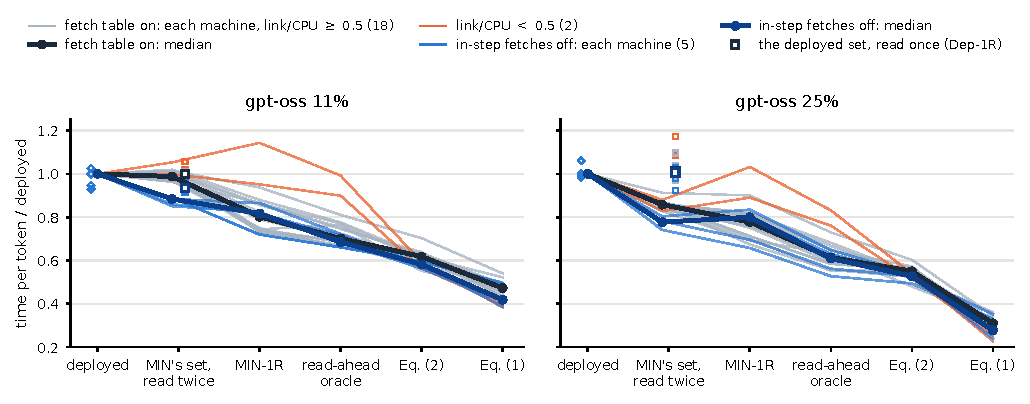
\includegraphics[width=0.88\textwidth]{figs/decomp_measured.pdf}
\caption{Where the seconds go, measured: each state's time per token relative to the deployed cache on the same
machine (lower is faster), as oracles change what is cached and how it is read (alone, then together) and when it is
read, with the two bounds for reference. One line per machine. Blue and orange: the panel, split at a link-to-CPU ratio
of 0.5; on the two slow-link machines (orange), reading once in the step saves little or costs time. Green: the
machines of the registered test. Thick dark lines: medians over the fast-link panel machines, changing MIN's set first
(solid) or the number of reads first (dashed).}
\label{fig:staircase}
\end{figure*}
% generated by scripts/decomp_measured.py
\begin{table}[!t]\centering\footnotesize
\caption{Where the deployed cache's time beyond \cref{eq:limit} goes, measured by removing each part in the engine (\cref{fig:staircase}): mean share of the gap over the 13 machines whose link reads at least 0.5 of their CPU rate, with 95\% intervals over machines. The first two parts are split order-free over the four combinations of what is cached and how it is read; $T_{\text{GPU}}$ is profiled, the rest measured.}\label{tab:gap}
\setlength\tabcolsep{3pt}\begin{tabular}{@{}p{0.52\linewidth}rr@{}}\toprule
Part of the gap & gpt-oss 11\% & 25\% \\\midrule
What is cached: MIN's set instead of the deployed one & 20\% [16, 23] & 29\% [27, 31] \\
How it is read: each admission read once, not twice & 19\% [16, 23] & 7\% [3, 10] \\
When it is read: copies issued a few steps ahead & 15\% [11, 18] & 20\% [18, 22] \\
GPU's non-expert work in series with the reads ($T_{\text{GPU}}$) & 27\% [24, 29] & 33\% [30, 36] \\
Left above \cref{eq:demand} with full foresight & 20\% [15, 25] & 11\% [7, 15] \\
\bottomrule\end{tabular}\end{table}

% generated by scripts/job112.py
\begin{table}[t]\centering\footnotesize
\caption{When the copy lands, against how often the expert is read: MIN's fewest-admission set read once (\FewOne), read twice with the copy published two steps after the admission (\FewTwo), and read twice with each copy issued a step earlier so that it lands for the next use (\FewEarly). Speed relative to the deployed cache on the same machine (95\% interval over problems as a subscript) and host misses per token, at gpt-oss 11\%; registered before the machines were rented.}\label{tab:timing}
\setlength\tabcolsep{2.5pt}\begin{tabular}{@{}lrrrrrrr@{}}\toprule
 & & \multicolumn{3}{c}{Speed vs deployed} & \multicolumn{3}{c}{Misses per token} \\\cmidrule(lr){3-5}\cmidrule(l){6-8}
Machine & Ratio & \cfg{1R} & \cfg{2R} & \cfg{2R-early} & \cfg{1R} & \cfg{2R} & \cfg{2R-early} \\\midrule
\multicolumn{8}{@{}l}{\emph{RTX 5090}} \\
Ryzen 9 7945HX & 0.88 & 1.25$_{\pm.01}$ & 1.03$_{\pm.00}$ & 1.00$_{\pm.00}$ & 40.7 & 55.7 & 54.6 \\
\bottomrule\end{tabular}\end{table}


\paragraph{On this engine, what is cached and how it is read pay only together.} At gpt-oss 11\%, \MinTwo, MIN's set on the deployed read path, closes \dmAllSetaloneLow\% of the gap, and
\DepOne, the deployed set read once, closes \dmAllOncealoneLow\%. \MinOne, both changes, closes \dmAllTogetherLow\% on the
panel and \dmNewTogetherLow\% on the new machines. MIN's set admits more experts than the deployed one, and on the
deployed path each extra admission costs a second read. Its copies also land two steps after the admission, so
\MinTwo{} misses more than \MinOne: the factor is the read path, which sets both the number of reads and when a copy
lands. A registered control tried to separate the two (\cref{tab:timing}): \FewEarly{} issues each copy of MIN's
fewest-admission set one step earlier, so that it lands for the next use. It failed its own check. Its misses fell only
to \tcMissRatioLowRng{} of \FewTwo's (registered: at most 0.95), because the fetch table still fills slots the schedule
did not choose, and it admitted \tcAdmEarlyLowRng{} experts per token against \FewTwo's \tcAdmTwoLowRng, reading
\tcHostEarlyPctLowRng\% more from the host. On \tcNWord{} machines at 11\% it ran \tcEarlyLowRng$\times$ the deployed
cache, \FewTwo{} \tcTwoLowRng$\times$ and \FewOne{} \tcOneLowRng$\times$. So the control cannot say how much of the
two-read arms' loss is late landing; it shows only that issuing the copies earlier, in this engine, does not recover it.
We registered a positive interaction on every machine: it was positive on \dmRegHeld{} of the \dmRegN{} machines of
the panel's main job (failed) and on all \dmNewInteractionPosLow{} new machines (held, on the point estimate). The claim is about MIN's greedy
set: its fewest-admission set read twice gains a little alone (\FewTwo, \tcTwoLowRng$\times$ on the control's machines)
and more on slow links (\cref{sec:secondcard}). At 25\%, where admissions are fewer, MIN's set alone already closes
\dmAllSetaloneMid\%.

\paragraph{What is left.} The read-ahead oracle closes another \dmAllAheadLow\% at 11\%, and \dmAllLeftLow\% of the gap
remains (\cref{tab:gap}). On fast links, two named parts account for it (at 25\% they slightly overshoot). The oracle still reads its remaining misses after their router
runs, so the GPU's non-expert time stays in series with them, and it reads more than MIN, because its early copies
evict sooner. A system that issued every read before routing and read no more than MIN would remove both, but only copies
over the link can be issued early (\cref{eq:dep}). On slow links the two parts fall short: a residual of
\dmSlowResidLowMin--\dmSlowResidLowMax\% of the gap at 11\% stays unexplained on the two slow-link panel machines, and
\cxResidLowMin--\cxResidLowMax\% on the three slow-link RTX 4090s of \cref{sec:secondcard}
(\cxResidOwnLowMin--\cxResidOwnLowMax\% with that card's own non-expert time). Of the gap to \cref{eq:dep}, the tighter
bound there, the read-ahead oracle still leaves \dmEqThreeLeftSlowLowMin--\dmEqThreeLeftSlowLowMax\% on the two
slow-link panel machines and \dmEqThreeLeftCardLowMin--\dmEqThreeLeftCardLowMax\% on the three RTX 4090s (median
\dmEqThreeLeftFastLowMed\% on fast links): the oracles fetch over the link, the slow path on these machines.

\section{How Foresight Must Be Spent}\label{sec:foresight}
This section measures each way of spending foresight as a speed relative to the deployed cache on the same machine. A
running example: on a Ryzen 9 9950X at gpt-oss 11\%, \cref{eq:limit} gives \slExBoundMs\,ms per token and
\cref{eq:demand} \slExDemandMs. The deployed cache takes \fsExBaseMs\,ms, \MinOne{} \fsExFetchMs, and the read-ahead
oracle \fsExPacedMs.

\begin{figure*}[t]\centering
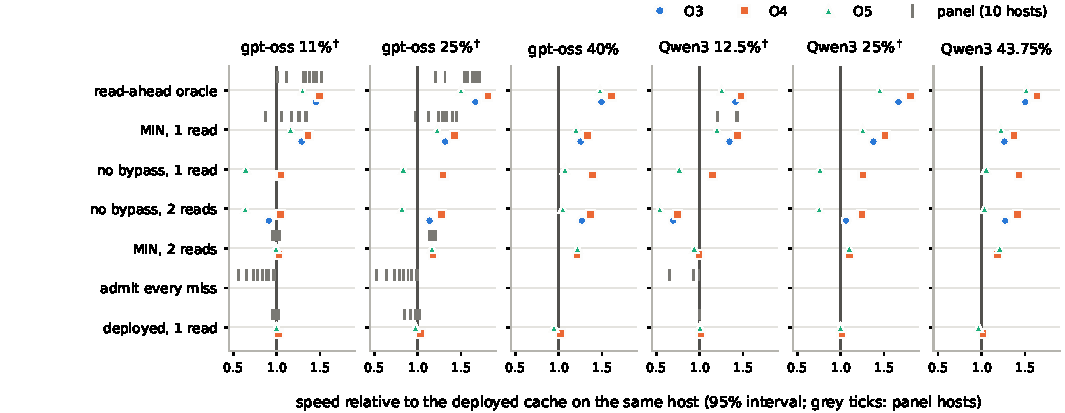
\includegraphics[width=0.9\textwidth]{figs/factorial.pdf}
\caption{What foresight is worth, by how it is spent: speed of each configuration of \cref{tab:configs} relative to the
deployed cache on the same machine, at the six budgets ($^\dagger$host-bound). Three machines at every budget (O3--O5:
two Ryzen 9 9950X and a 9950X3D); the \pnHosts{} machines of the panel's main job (grey ticks) at the two host-bound gpt-oss budgets, and
\pnHostsQlow{} of them at Qwen3 12.5\%. \MinOne{} gains at every budget on these machines; reading twice or
admitting what MIN bypasses gains at some budgets and loses at others.}
\label{fig:factorial}
\end{figure*}

\paragraph{Read each admitted expert once.} \MinOne{} is
faster than the deployed cache at every budget on the three factorial machines (\cref{fig:factorial}). The usual ways of
spending foresight waste reads. Prefetching without bypass, Belady's original rule, admits experts MIN would bypass.
Serving a miss on the CPU before copying it reads every admission twice. At the smallest budget of each model these gain
at most \fxUsualLowGainMax\% or lose, a trade-off known for disks \citep{cao1995prefetching} and CPU caches
\citep{jain2018prefetch}. (Registered as gain bands per budget on two machines; held at most budgets.)

\paragraph{Admit as rarely as optimality allows.} The greedy schedule
admits whenever MIN allows and may evict an expert again before its next use. The fewest-admission schedule makes
\jfCopyRatioMin--\jfCopyRatioMax{} of the greedy one's copies for the same hits in replay. Read once in the step at
gpt-oss 11\% (\FewOne), it beat the deployed cache on all \rbPlanMachines{} machines that ran it stably, by a geometric
mean of \rbPlanMean$\times$ (registered on \rbPlanRegMachines{} of them; \rbPlanCardTwo{} are RTX 4090s and \rbPlanServer{}
have server processors). Counting the machines that ran unsteadily as well, it lost on \rbPlanUnstLost{}, the two with
the slowest links (ratios \rbPlanLostRatios; \cref{app:more}): the stability rule leaves out exactly those.

\section{Without Foresight, the Engine Recovers Little}\label{sec:online}
Two of the engine's mechanisms act on the same levers without foresight, in four variants (\cref{tab:configs}).
\Margin{} admits less: it cuts the deployed cache's host reads by \jiDkReadsGLowMin--\jiDkReadsGLowMax\% at 11\%. \LA{}
copies, one layer ahead, the expert that the next layer's router predicts, so that a correctly predicted admission is
read once, by the GPU; \LAOne{} and \LAOneM{} also fetch every admission in the step. We registered that none of the
four would run faster than 1.10$\times$ the deployed cache or capture more than 35\% of the read-ahead oracle's gain on
any machine; the second threshold was loose. At 11\% the best of them runs \olBestLowMin--\olBestLowMax$\times$ the
deployed cache, at most \olCapLowMax\% of the read-ahead oracle's gain. The counters say why: the four read
\olReadsFourLowMin--\olReadsFourLowMax$\,R^\star$ host experts per token, about as many as the deployed cache. A prediction
one layer ahead moves reads earlier but does not avoid them. On the slow-link RTX 4090s of \cref{sec:secondcard}, the
variants built on the layer-ahead copy lose time (\cxLayerLowMin--\cxLayerLowMax$\times$ at 11\%), as registered, and
\Margin{} is the best, at \cxBestLowMin--\cxBestLowMax$\times$: up to \cxCapLowMax\% of an oracle gain that is smaller
there.

% generated by scripts/job109.py
\begin{table*}[t]\centering\footnotesize
\caption{The registered tests on machines rented for them: speed relative to the deployed cache on the same machine (geometric mean of its rounds) of \MinOne, the read-ahead oracle (\emph{ahead}), and the best of the four variants without foresight (\emph{none}: \Margin, \LA, \LAOne, \LAOneM; \cref{sec:online}), and that variant's capture, its share of the read-ahead oracle's gain. \emph{Ratio}: link-to-CPU. RTX 5090: job 109, whose population (desktop-class, link-to-CPU ratio at least 0.5) was fixed before any machine started. RTX 4090: job 111 (job 110's predictions, committed before any RTX 4090 ran); in brackets, what the RTX 5090 machines' trend in the link-to-CPU ratio predicted for that machine. Subscripts: half-width of the 95\% interval over problems (paired bootstrap within the machine).}\label{tab:job109}
\setlength\tabcolsep{3pt}\begin{tabular}{@{}lrrrrrrrrr@{}}\toprule
 & & \multicolumn{4}{c}{gpt-oss 11\%} & \multicolumn{4}{c}{gpt-oss 25\%} \\\cmidrule(lr){3-6}\cmidrule(l){7-10}
Machine & Ratio & \MinOne & Ahead & None & Capture & \MinOne & Ahead & None & Capture \\\midrule
\multicolumn{10}{@{}l}{\emph{RTX 5090, job 109}} \\
Core Ultra 9 285K & 0.54 & 1.22$_{\pm.01}$ & 1.46$_{\pm.01}$ & 1.02$_{\pm.00}$ & 4$_{\pm0}$\% & 1.24$_{\pm.01}$ & 1.64$_{\pm.02}$ & 1.03$_{\pm.00}$ & 4$_{\pm0}$\% \\
Core i9-13900KF & 0.59 & 1.25$_{\pm.01}$ & 1.46$_{\pm.01}$ & 1.01$_{\pm.00}$ & 2$_{\pm0}$\% & 1.26$_{\pm.01}$ & 1.61$_{\pm.02}$ & 1.01$_{\pm.01}$ & 2$_{\pm1}$\% \\
Ryzen 9 5950X & 0.84 & 1.37$_{\pm.01}$ & 1.50$_{\pm.01}$ & 1.01$_{\pm.00}$ & 2$_{\pm0}$\% & -- & -- & -- & -- \\
Ryzen 7 9800X3D & 0.88 & 1.15$_{\pm.01}$ & 1.34$_{\pm.01}$ & 1.01$_{\pm.01}$ & 4$_{\pm2}$\% & 1.22$_{\pm.01}$ & 1.55$_{\pm.02}$ & 1.01$_{\pm.00}$ & 2$_{\pm1}$\% \\
Ryzen 9 7945HX & 0.89 & 1.24$_{\pm.01}$ & 1.42$_{\pm.01}$ & 1.02$_{\pm.01}$ & 6$_{\pm1}$\% & 1.28$_{\pm.01}$ & 1.63$_{\pm.02}$ & 0.99$_{\pm.01}$ & $-$1$_{\pm1}$\% \\
\addlinespace
\multicolumn{10}{@{}l}{\emph{RTX 4090, job 111}} \\
Core i9-14900KF & 0.37 & 0.96$_{\pm.00}$ {\scriptsize[0.99]} & 1.13$_{\pm.01}$ {\scriptsize[1.11]} & 1.03$_{\pm.00}$ & 26$_{\pm3}$\% & 1.02$_{\pm.00}$ {\scriptsize[1.07]} & 1.30$_{\pm.01}$ {\scriptsize[1.29]} & 1.04$_{\pm.00}$ & 13$_{\pm1}$\% \\
Core Ultra 9 285K & 0.39 & 1.01$_{\pm.00}$ {\scriptsize[1.01]} & 1.20$_{\pm.01}$ {\scriptsize[1.13]} & 1.04$_{\pm.00}$ & 20$_{\pm2}$\% & 1.06$_{\pm.01}$ {\scriptsize[1.09]} & 1.36$_{\pm.01}$ {\scriptsize[1.31]} & 1.04$_{\pm.00}$ & 12$_{\pm1}$\% \\
Core Ultra 9 285K & 0.40 & 1.01$_{\pm.00}$ {\scriptsize[1.01]} & 1.20$_{\pm.01}$ {\scriptsize[1.13]} & 1.04$_{\pm.00}$ & 20$_{\pm2}$\% & 1.06$_{\pm.01}$ {\scriptsize[1.09]} & 1.37$_{\pm.01}$ {\scriptsize[1.32]} & 1.05$_{\pm.00}$ & 12$_{\pm1}$\% \\
\bottomrule\end{tabular}\end{table*}


\section{The Link-to-CPU Ratio on a Second Card}\label{sec:secondcard}
On the RTX 5090 machines, the gain of every configuration that moves reads from the CPU to the link follows the
link-to-CPU ratio: for \MinOne, Spearman \rcFetchRatio{} [\rcFetchRatioLo, \rcFetchRatioHi] over the \rcFetchRatioN{}
machines of jobs 093--104 (\cref{fig:hostdep}). We froze that trend on the \dmMachines{} panel machines, one line in the log of the ratio
for each of \MinOne, \MinTwo, \DepOne{} and the read-ahead oracle, and registered that their speed on RTX 4090 machines,
a slower card behind a PCIe 4.0 link, would fall within 0.10 of it in log. The first test ran on \cxNWord{} machines,
all at ratios \cxRatioMin--\cxRatioMax; a second, with the same predictions, added \tcFourNWord{} at
\tcRatioFourRng. On all \cxAllNWord, \MinOne{} and the read-ahead oracle came within \cxAllDevLowMax\% of the
prediction at 11\% and \cxAllDevMidMax\% at 25\% (\cref{tab:job109}), and every machine's 95\% interval over problems
lies inside the band; the interaction of \cref{sec:gap} is positive on the \tcFourFastN{} with fast links, as
registered. (The first test was relaunched with the RTX 4090's own reference loss; \cref{app:prereg} gives the
first rounds.) Predicting no change would have missed by up to \cxNoChangeDevLowMax\% at 11\% and
\cxNoChangeDevMidMax\% at 25\%. Applied after the fact to the new RTX 5090s of \cref{sec:gap}, all fast-linked, the
same trend misses \olTrendMissWord{} of their \olTrendCells{} cells by more than the band, by up to \olTrendDevMax\%:
on fast links the ratio sets the direction of the gain more reliably than its size. Where the link reads at under a
third of the CPU rate, \FewTwo{} pays instead of \MinOne{} (\jkSlowBypassPlanMin--\jkSlowBypassPlanMax$\times$ over the two
budgets on RTX 5090s at ratios \jkSlowRatioMin--\jkSlowRatioMax).

\begin{figure*}[t]\centering
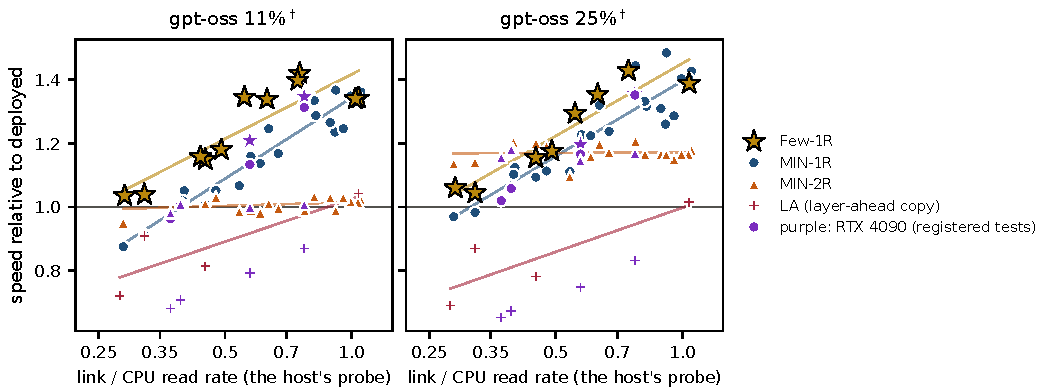
\includegraphics[width=0.86\textwidth]{figs/hostdep.pdf}
\caption{The machine decides which way of spending foresight pays: speed relative to the deployed cache on the same
machine against the machine's link-to-CPU ratio, at the two host-bound gpt-oss budgets. Every marker is a machine that
passed our checks. Stars: \FewOne. Circles and triangles: \MinOne{} and \MinTwo, both on the greedy schedule. Crosses:
\LA. Purple markers: the RTX 4090 machines of the registered second-card test (\cref{sec:secondcard}), not used in the fits.
Lines: least-squares fits in the log of the ratio, drawn for the trend only.}
\label{fig:hostdep}
\end{figure*}

\section{How Much Foresight Is Needed}\label{sec:horizon}
The oracles know the whole future; a predictor would know part of it, imperfectly. We give the cache a \emph{window},
the routing of the next $W$ tokens, exact or with each future expert right only with probability $r$. Throughout this
section, the value of a window is its share of MIN's gain over admitting every miss, the online policy that reads least
at these budgets (\cref{app:value} gives the policies).

\begin{figure*}[t]\centering
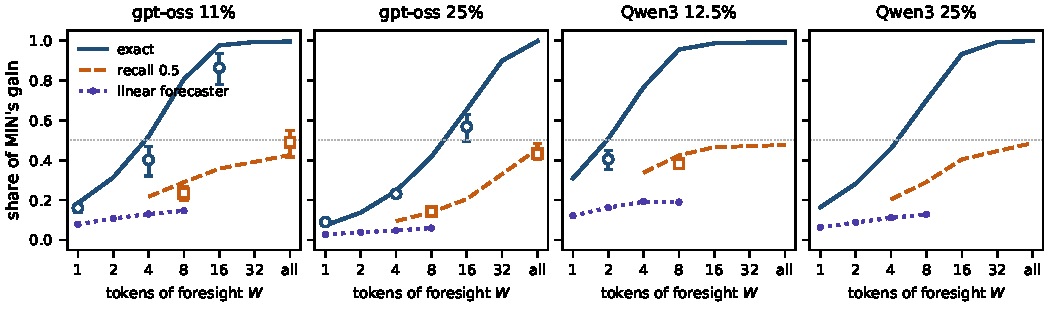
\includegraphics[width=0.8\textwidth]{figs/value.pdf}
\caption{Baseline here: \emph{admit every miss}, not the deployed cache. The share of MIN's gain over admitting every
miss recovered, in host reads on the routing the engine runs, by exact routing of the next $W$ tokens (solid), by a
window whose experts are each right with probability 0.5 (dashed) and by a linear forecaster fitted on other text
(dotted). Markers: the same share in time per token (mean and range over the panel's main-job machines: \pnHostsLow{}
for gpt-oss, \pnHostsQlow{} for Qwen3 12.5\%). Grey line: half of the gain.}
\label{fig:value}
\end{figure*}

\paragraph{Next-token prediction buys little.} Exact routing of the next token recovers at most \vmShareOneQlow{} of
MIN's gain at any host-bound budget of our two models; half of the gain at gpt-oss 11\% needs \vmHalfLow{} tokens
(\cref{fig:value}). In the engine, an exact 16-token window recovers \pnShareSixteenLowMin--\pnShareSixteenLowMax{} of
the gain in time at 11\% (registered at 0.80 or more; the lowest machine missed). Against the deployed cache, the
same window copied in the step runs \jaWSixteenLowMin--\jaWSixteenLowMax$\times$ at 11\% on \jaHosts{} machines, below 1
on the \jaPathLowN{} with the lowest link-to-CPU ratios. Accuracy matters as much as horizon: an 8-token window that
is right half the time recovers \vmEightHalfLow{} of the gain at 11\%, about what 2 exact tokens buy (\vmShareTwoLow).

\paragraph{The horizon is measured in distinct experts (exploratory).} On \fsModels{} models' own sampled text, the
window that closes half of the read gap ranges from \dcWMin{} to \dcWMax{} tokens. Paging theory measures lookahead in
distinct pages \citep{albers1997lookahead,breslauer1995lookahead}, and so does the rule that fits: within that window a
layer requests about \dcMed$\,C$ distinct experts (\dcAimeMin--\dcAimeMax$\,C$ on the AIME routing the engine
runs). Given a model's routing trace, this one-constant rule predicts its horizon
as well as a two-constant power law in tokens (\cref{app:traces}).

\paragraph{Nothing realisable reaches it.} Forecasters trained on routing histories, linear or recurrent, close at
most \lfShareMaxGpt\% of the read gap on gpt-oss: their precision falls with the horizon. Speculative batches save an
online cache about a tenth of its reads at 90\% draft acceptance and cost reads at 80\%
\citep{spmoe,moespac2026,cascade2025} (\cref{app:traces}). Layer-ahead predictors
\citep{hwang2024pregated,zhu2025preattention} reach \laRecallK\% recall in our engine but see less than one token
ahead (\cref{sec:online}).

\section{What This Means for System Builders}\label{sec:builders}
These rules come from one engine (ours), batch-1 decode and one prompt set, and rules 2--4 from one model at two budgets;
elsewhere they are hypotheses to test, with \cref{eq:limit} as the yardstick.
\begin{enumerate}\setlength\itemsep{1pt}
\item \textbf{Report the distance to the machine's bound.} A speed-up over a chosen baseline hides how much is left.
\Cref{eq:limit} needs only the routing trace and one probe run.
\item \textbf{Change what is cached and how it is read together.} Serving a miss on the CPU and then copying it into a
slot reads it twice. At the smallest budget, a better set read twice, or the same set read once, closes almost none of the gap; where the link reads at least half as
fast as the CPU, a better set read once closes about a third of it.
\item \textbf{Do not expect a policy without foresight to get there.} Admitting less and predicting one layer ahead
recover at most \olCapLowMax\% of what foresight is worth where it is worth most, and the layer-ahead copy loses time on
slow links; the reads they leave are the ones only foresight avoids.
\item \textbf{Choose the read path by the link-to-CPU ratio.} Where the link is fast, copy misses into slots in the
step; where it is slow, serve them on the CPU and copy in the background. The ratio predicts the direction of the
gain more reliably than its size (\cref{sec:secondcard}).
\item \textbf{Issue reads before routing, and predict far enough ahead to save reads.} Even with full foresight, the
GPU's non-expert time stays in series with every read that waits for the router; only a prediction lets reads
start earlier, and only over the link (\cref{eq:dep}). To save reads, predictors should target the next
$\approx$\dcMed$\,C$ distinct experts of each layer, not the next token; accuracy counts as much as horizon.
\end{enumerate}

\section{Related Work}\label{sec:related}
\paragraph{Offloading systems.} Expert caches copy misses over PCIe
\citep{eliseev2023offloading,xue2024moeinfinity,song2024promoe,tang2024hobbit}; CPU-execution systems run non-resident
experts on the host \citep{kamahori2024fiddler,ktransformers,zhong2025hybrimoe,daop2025}; FreeToken \citep{freetoken} and DALI \citep{dali2026} split each layer's misses between the two. Predictors guess
upcoming experts from the previous layer \citep{hwang2024pregated,zhu2025preattention}, several tokens ahead
\citep{wang2026seqmoe,mira2026}, from draft tokens \citep{spmoe,moespac2026,cascade2025}, or decouple the router
\citep{readme2024}. Each reports speed-ups over its own baseline; none bounds the machine. \Cref{app:related} covers these and many
more, with batched and flash-tier systems.

\paragraph{Bounds and caching theory.} WiSP \citep{wisp2026}, Budgeting Bytes \citep{budgetingbytes2026}, MoE-CAP
\citep{moecap} and the roofline \citep{williams2009roofline} bound decode by bytes over bandwidth;
\citet{zhang2026reproducible} and \citet{liang2026lrc} compare caches with MIN in hits. We add the time domain. MIN
with bypass maximises hits \citep{carlisle1995kcoloring,jain2016hawkeye}, not speed \citep{bypassopt}; our
fewest-admission schedule extends offline caching over reuse intervals \citep{berger2018foo}.

\section{Limitations}\label{sec:limits}
\begin{itemize}\setlength\itemsep{1pt}
\item \textbf{Hardware, engine, sample and workload.} One engine, ours, for every engine result; one GPU model for most results and a second (RTX 4090) for two
registered tests, all rented, mostly in desktop hosts; clocks could not be locked; batch-1 decode of two models on AIME
prompts, also used while developing the system, teacher-forced on each model's own greedy text. The first RTX 4090 test deviated from its registration,
and the last experiment replaced one machine early (\cref{app:prereg}); where the crossovers between read paths lie
rests on few slow-link machines. The machines are a convenience sample of the cheapest offers that passed our checks,
and rented machines are often shared or unsteady (of \jmServAll{}
launches on server processors only \jmServWord{} passed every check).
\item \textbf{The bounds.} Exact routing and per-layer slots; pooling slots across layers lowers MIN's reads by
\globalReadsMin--\globalReadsMax\%. The bounds drop latencies and are relative to one run of our probe, mostly taken
while the model downloaded: the engine's reads imply a rate more than 5\% above the probe's highest reading on
\rbAboveMax{} of \rbLaunchBudgets{} launch-budgets (\cref{tab:robust}). A second probe on the idle machine came within
\tcProbeDevMax\% of the first on \tcProbeN{} machines, but between two rentals of one machine the ratio moved by up to
\tcRelaunchRatioDevMax\%. $T_{\text{GPU}}$ is our engine's kernel time on an RTX 5090.
\item \textbf{The decomposition and the oracles.} The parts are measured at two budgets of one model; what the oracles
leave is split by attribution, not measurement. Oracles read a recorded trace, and on the two-read path the engine
does not keep MIN's set (\cref{sec:gap}). The engine's only predictor looks one layer ahead; the forecasters of
\cref{sec:horizon} were evaluated offline.
\item \textbf{Outputs and more.} Parity is measured by teacher-forced KL divergence against an all-VRAM reference (mean
\klMeanGpt{} and \klMeanQwen{} nats), not by task accuracy; \cref{app:limits} gives the remaining caveats.
\end{itemize}

\section{Conclusion}
MIN's host reads at a machine's probed rate bound batch-1 MoE decode from host memory, and our cache reaches
\dcShareMinLowMin--\dcShareMinLowMax\% of that bound at the smallest gpt-oss budget. In our engine, what is cached pays
only when each admitted expert is read once, and policies without foresight recover little of the rest.
